\documentclass[xcolor=pdftex,dvipsnames,table,aspectratio=169]{beamer}
%\documentclass[xcolor=pdftex,dvipsnames,table,handout,aspectratio=169]{beamer}

%\setbeameroption{show notes}

\usepackage{bm,graphicx,multirow,amsmath,tikz} %fancybox,
\usepackage{color}%,textpos}
\usepackage[round]{natbib}
\usepackage[normalem]{ulem}
\usepackage{hyperref}
\usepackage{lastpage}
\usepackage{array}
\usepackage{color}
\usepackage{framed}
\usepackage{hyperref}

% Define Western colours
\definecolor{western}{rgb}{.306,.152,.524}
\definecolor{westerngray}{rgb}{.512,.508,.524}

%% Define BEAMER colours
\setbeamercolor{frametitle}{bg=western,fg=white}
\setbeamercolor{framesubtitle}{bg=western,fg=black}
\setbeamercolor{title}{fg=white,bg=western}
\setbeamercolor{author}{fg=white,bg=western}
\setbeamercolor{institute}{fg=white,bg=western}
\setbeamercolor{date}{fg=white,bg=western}

%% Set BEAMER fonts
\setbeamerfont{title}{shape=\bf}
\setbeamerfont{frametitle}{shape=\sc,size=\Large}
\setbeamerfont{framesubtitle}{shape=\sc,size=\Large}
\setbeamerfont{footline}{shape=\sc}

%% Define BEAMER toc
\setbeamercolor{section in toc}{fg=western}
\setbeamercolor{subsection in toc}{fg=westerngray}
\setbeamertemplate{sections/subsections in toc}[ball]

%% Define BEAMER background
\setbeamercolor{background canvas}{bg=white}

%% Define BEAMER footer
\setbeamertemplate{navigation symbols}{}
\setbeamercolor{footline}{fg=white,bg=western}
\setbeamertemplate{footline}{%
  \begin{beamercolorbox}[wd=\paperwidth]{footline}
    \vskip5pt

    \raisebox{.05in}{
      \scriptsize{\bf \insertshorttitle}
    }
    \hfill
    \raisebox{.05in}{
      \scriptsize{\bf \insertframenumber/\inserttotalframenumber} 
    }
    \hspace{5pt}

    \vskip5pt
  \end{beamercolorbox}
}

%% Define BLOCK environment
\setbeamercolor{block title}{fg=western}
\setbeamerfont{block title}{series=\bfseries}

%% Define ENUMERATE and ITEMIZE environements
\setbeamertemplate{itemize item}[ball]
\setbeamertemplate{enumerate item}[ball]
\setbeamercolor{item projected}{bg=western}

%% Define BEAMER toc
\setbeamercolor{sections/subsections in toc}{fg=blue!75}
\setbeamertemplate{sections/subsections in toc}[ball]

% %% Define SECTION openings
% \AtBeginSection[]{
%   \begin{frame}{\insertshorttitle}
%     \tableofcontents[currentsection,subsectionstyle=hide/hide/hide]
    
%   \end{frame}
% }

%% Define BEAMER frametitle
\addtobeamertemplate{frametitle}{
   \let\insertframetitle\insertsectionhead}{}
\addtobeamertemplate{frametitle}{
   \let\insertframesubtitle\insertsubsectionhead}{}


\makeatletter
  \CheckCommand*\beamer@checkframetitle{\@ifnextchar\bgroup\beamer@inlineframetitle{}}
  \renewcommand*\beamer@checkframetitle{\global\let\beamer@frametitle\relax\@ifnextchar\bgroup\beamer@inlineframetitle{}}
\makeatother

% Define counters for example and exercise
\newcounter{example}
\newcounter{exercise}

% Define example and exercise commands
\renewcommand{\example}
{\stepcounter{example}Example \lecturenum.\arabic{example}}
\newcommand{\examplectd}
{Example \lecturenum.\arabic{example}\ ctd}
\newcommand{\exercise}
{\stepcounter{exercise}Exercise \lecturenum.\arabic{exercise}}
\newcommand{\exercisectd}
{Exercise \lecturenum.\arabic{exercise}\ ctd}

\newcommand{\lecturenum}{8}

\title[SS2857 -- Lecture 8]{SS2857 Probability and Statistics 1\\
  Fall 2021\\
  \vspace{.2in}
  Lecture 8}

\date{Revised 02/10/24}

%% Initialize R


\begin{document}

{
\setbeamertemplate{footline}{}
\setbeamercolor{background canvas}{bg=western}

\begin{frame}
  \addtocounter{framenumber}{-1}

  \maketitle
\end{frame}
}

\section{Probability Distributions for Discrete RVs}

\begin{frame}
  \frametitle{\invisible{Hello}}

  \begin{center}
    \Large{\textbf{3.2 Probability Distributions for Discrete Random Variables}}
  \end{center}

\end{frame}

\begin{frame}
  \begin{block}{Probability Distribution}
  The probability distribution (aka the distribution) of a random variable identifies:
  \begin{enumerate}[1)]
  \item The possible values of the random variable.
  \item How the probability is distributed to these values.
  \end{enumerate}
  \end{block}
\end{frame}

\begin{frame}
  \begin{block}{Probability Mass Function}
    The probability mass function (pmf) of a discrete random variable is the function
    \[
      p(x)=P(X=x), x \in \mathbb X.
    \]

    \pause
    
    \medskip

    Probability mass functions may either be defined as a function or in a table.

    \medskip


    \pause 
    
    We commonly define the probability mass function where it is positive and implicitly assume that the function is equal to zero for all other values. E.g.,
    \[
      p(x)=P(X=x)=.5, x \in \{0,1\}
    \]
    implies $P(X=x)=0$ for all other $x \in \mathbb R$. 
    
  \end{block}
\end{frame}

\begin{frame}

  \begin{block}{\example: Probability Mass Functions}

    Approximately 79\% of world's population has brown eyes. 
    
    \bigskip
    
    Suppose that we sample 5 people from the population at random with replacement and record their eye-colour as brown or not brown. Let $X$ be the number of people in our sample with brown eyes.
    
    \bigskip

    \begin{enumerate}[a)]
    \item Compute the pmf of $X$.
    \item Draw a figure showing the pmf of $X$. 
    \end{enumerate}
  \end{block}
\end{frame}



\begin{frame}
\begin{block}{\example: Probability Mass Functions}
% latex table generated in R 4.4.1 by xtable 1.8-4 package
% Wed Oct  2 15:17:47 2024
\begin{table}[ht]
\centering
\begin{tabular}{rr}
  \hline
x & $p(x)$ \\ 
  \hline
     0 & 0.00041 \\ 
       1 & 0.00768 \\ 
       2 & 0.05780 \\ 
       3 & 0.21743 \\ 
       4 & 0.40898 \\ 
       5 & 0.30771 \\ 
   \hline
\end{tabular}
\end{table}

\end{block}
\end{frame}

\begin{frame}

  \begin{block}{\examplectd: Probability Mass Functions}
    The pmf of $X$ looks like this:

    \begin{center}
      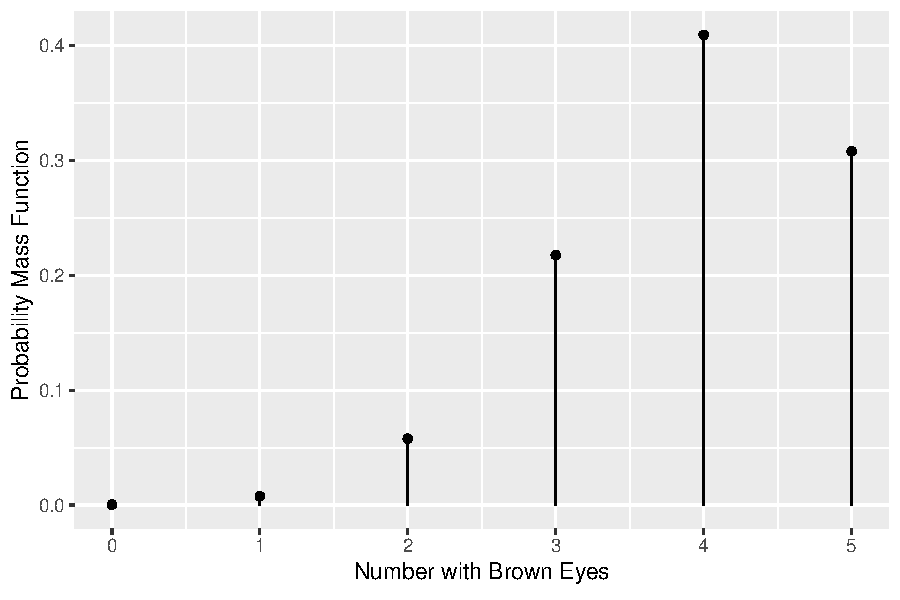
\includegraphics[height=.6\textheight]{figure/example10-1-1-1}
    \end{center}
  \end{block}
\end{frame}





\begin{frame}
  \begin{block}{Cumulative Distribution Function}
    The cumulative distribution function (cdf) of a discrete random variable is the function
    \[
      F(x)=P(X \leq x)=\sum_{y:y \in D, y \leq x} p(y), x \in \mathbb X.
    \]

    \pause
    
    \medskip

    Cumulative distribution functions may either be defined as a function or in a table.

    \medskip

    The cdf must be defined for all values along the real line. E.g.,
    \[
      F(x)=P(X \leq x)
      \left\{
        \begin{array}{ll}
          0 & x <0\\
          .5 & 0 \leq x < 1\\
          1 & x \geq 1.
        \end{array}
      \right.
    \]

  \end{block}
\end{frame}

\begin{frame}

  \begin{block}{\examplectd: Cumulative Distribution Functions}

    Approximately 79\% of world's population has brown eyes. 
    
    \bigskip
    
    Suppose that we sample 5 people from the population at random with replacement and record their eye-colour as brown or not brown. Let $X$ be the number of people in our sample with brown eyes.
    
    \bigskip

    \begin{enumerate}[a)]
    \setcounter{enumi}{3}
    \item Compute the cdf of $X$.
    \item Draw a figure showing the cdf of $X$. 
    \end{enumerate}
  \end{block}
\end{frame}

\begin{frame}

\begin{block}{\examplectd: Cumulative Distribution Functions}
$$
F(x)=\left\{
\begin{array}{ll}
0 & x < 0\\
p(0)=.00041 & 0 \leq x < 1\\
p(0) + p(1) = .00809 & 1 \leq x < 2\\
p(0) + p(1) + p(2) = .065989 & 2 \leq x < 3\\
p(0) + p(1) + p(2) + p(3) = .28332 & 3 \leq x <4\\
p(0) + p(1) + p(2) + p(3) + p(4)= .69229 &4 \leq x <5\\
p(0) + p(1) + p(2) + p(3) + p(4) + p(5)= 1 & 5 \leq x\\
\end{array}
\right.
$$
 \end{block}
\end{frame}


\begin{frame}

  \begin{block}{\examplectd:Cumulative Distribution Functions}

    \begin{center}
      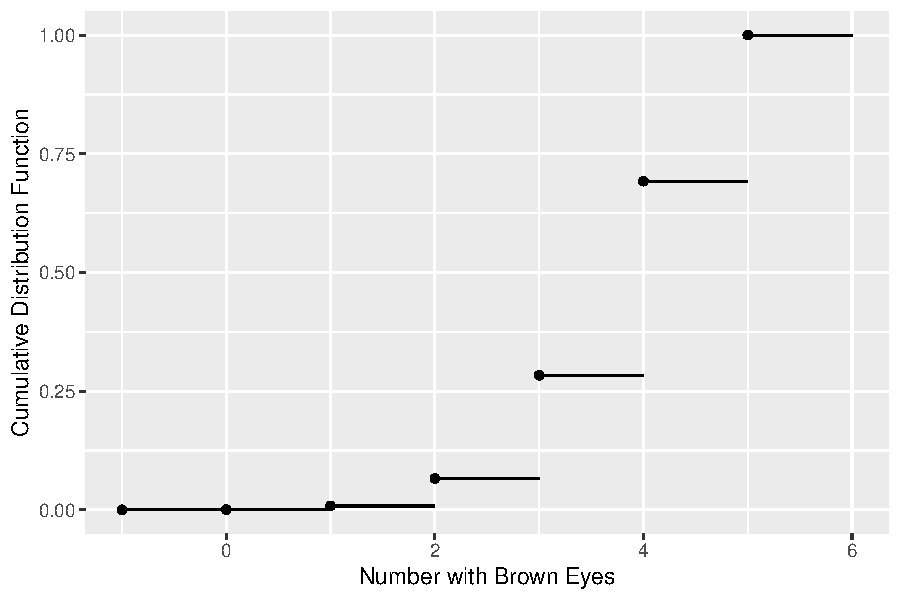
\includegraphics[height=.6\textheight]{figure/example-10-1-4-1}
    \end{center}
  \end{block}
\end{frame}



\begin{frame}
  \begin{block}{Cumulative Distribution Functions}

  Any cumulative distribution, $F(x)$, must satisfy the following properties:
  \begin{itemize}
  \item Tends to 0 as $x$ decreases: $\lim_{x \to -\inf}=0$.
  \item Tends to 1 as $x$ increases: $\lim_{x \to \inf}=1$.
  \item Non-decreasing.
  \item Continuous from the right: $\lim_{x^* \downarrow x} F(x^*)=F(x)$.
  \end{itemize}

  \bigskip

  Cumulative distributions for discrete random variables are step functions.
  \end{block}
\end{frame}

\begin{frame}
  \begin{block}{Parameter}
    A parameter is a quantity that can be assigned different possible values to identify one specific distribution within a family of distributions.

    E.g., the family of Bernoulli distributions is defined by the pmf
    \[
      p(x)=\left\{
        \begin{array}{ll}
          1-p &x=0\\
          p & x=1
        \end{array}
      \right.
      =p^x(1-p)^{\textcolor{red}{(1-x)}}.
    \]
    The parameter is $p$. 
  \end{block}
\end{frame}

\begin{frame}
  \begin{block}{\example}
    Let $p$ be the proportion of the world's population with brown eyes. 
    
    \bigskip

    Suppose that we sample 5 people from the population at random with replacement and record their eye-colour as brown or not brown. Let $X$ be the number of people in our sample with brown eyes.
    
    \bigskip

    How would the distribution of $X$ change if $p$ was varied between 0 and 1?
  \end{block}
\end{frame}

\begin{frame}

  \begin{block}{\examplectd}
    \begin{center}
      \begin{tabular}{cc}
        $p=.1$ & $p=.4$\\
        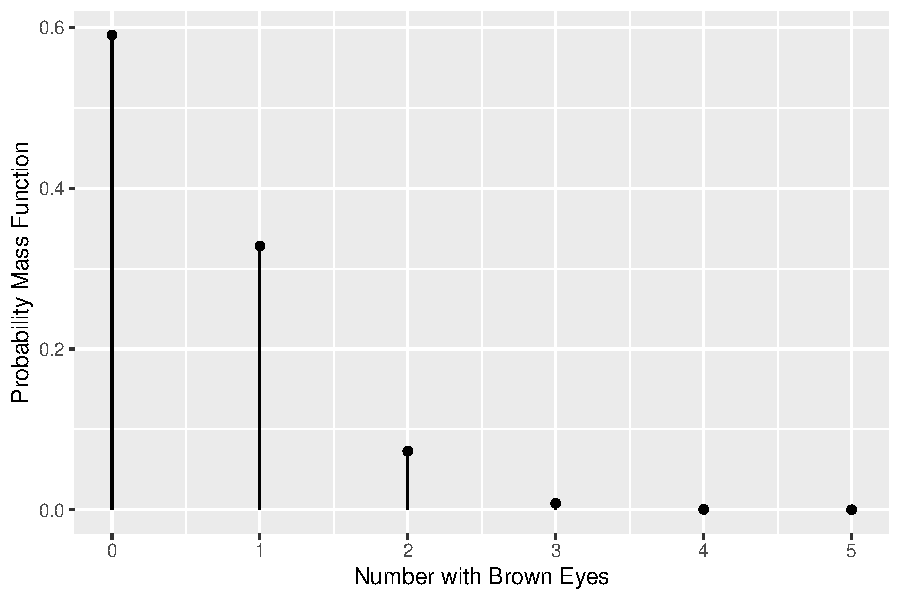
\includegraphics[height=.32\textheight]{figure/example-10-1-5-1} &
                                                                           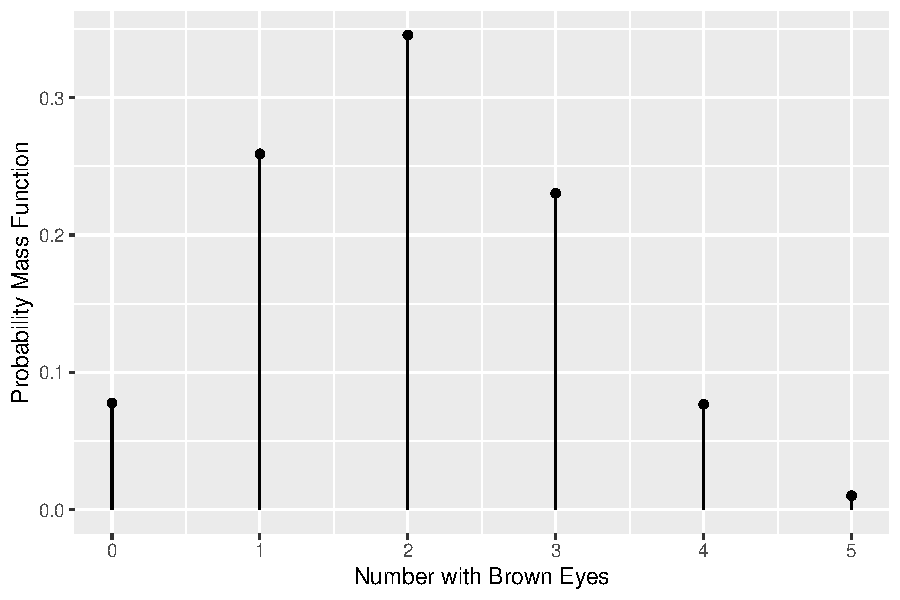
\includegraphics[height=.32\textheight]{figure/example-10-1-5-2} \\
        $p=.6$ & $p=.9$\\
        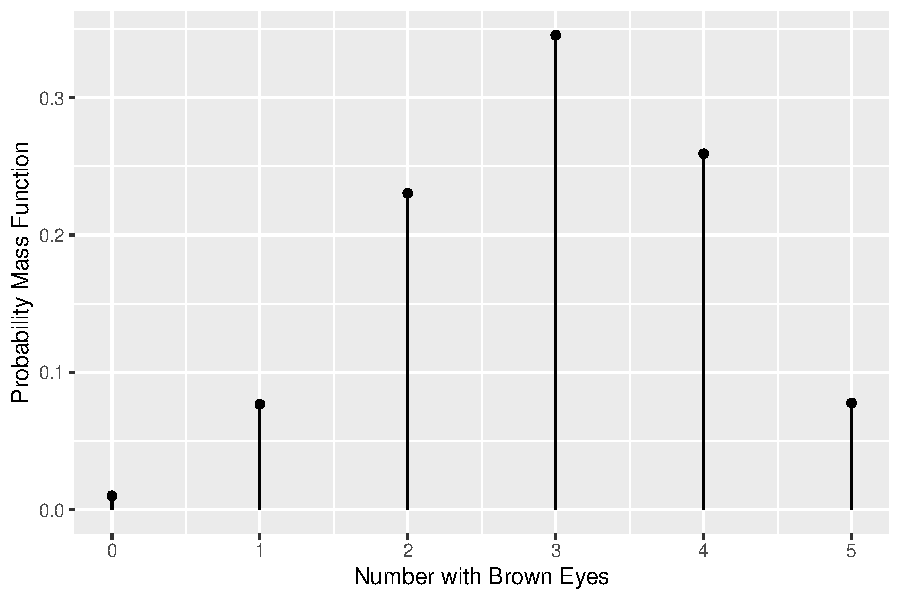
\includegraphics[height=.32\textheight]{figure/example-10-1-5-3} &
                                                                           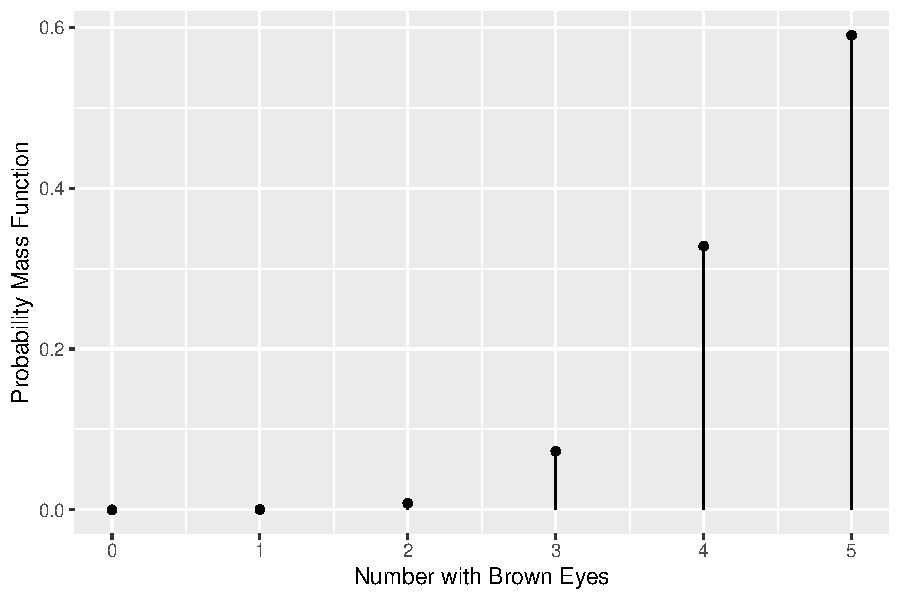
\includegraphics[height=.32\textheight]{figure/example-10-1-5-4} 
      \end{tabular}
    \end{center}
  \end{block}
\end{frame}

\begin{frame}

  \begin{center}
    \Large{\textbf{Questions?}}
  \end{center}
\end{frame}

\begin{frame}

\begin{block}{\exercise}
Consider a discrete random variable, Z, with the cdf:
$$
F(z)=
\left\{
\begin{array}{ll}
0 & x < 0\\
0.292  &   0 \leq x <1\\
0.745  &  1 \leq x <2\\
0.965  &  2 \leq x <3\\
0.998 &   3 \leq x <4\\
1     &    x \geq 4
\end{array}
\right.
$$
\end{block}

\begin{enumerate}[a)]
\item Sketch the cdf.
\item What are the possible values $Z$ (i.e., for what values of $z$ is $P(Z=z)>0$)?
\item What is the probability mass function?
\item Sketch the pmf.
\end{enumerate}
\end{frame}

\end{document}
